\subsubsection{UC1 - Caricamento file}
\begin{figure}[h]
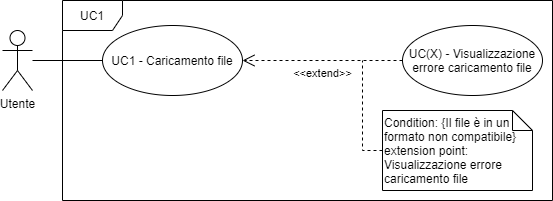
\includegraphics[width=\linewidth]{section/Images/UC1CaricamentoFile.png}
\centering
\caption{UC1 - Caricamento file}
\end{figure}
\begin{itemize}
	\item \textbf{Attore primario}: Utente.
	\item \textbf{Precondizioni}: Il sistema è raggiungibile e funzionante. L'utente è in possesso di un file contenente i dati che vuole inserire.
	\item \textbf{Postcondizioni}: Viene visualizzato un messaggio che avvisa l'utente del corretto caricamento del file e della sua validità. I dati presenti nel file vengono caricati nel sistema.
	\item \textbf{Scenario principale}:
		\begin{enumerate}
			\item L'utente accede al sistema;
			\item L'utente seleziona la funzionalità "carica file";
			\item L'utente seleziona il file da caricare.
		\end{enumerate}
	\item \textbf{Estensioni}:
	\begin{enumerate}[(a)]
		\item Nel caso in cui il file sia in un formato sbagliato:
		\begin{enumerate}[1.]
			\item i dati non vengono caricati nel sistema;
			\item viene visualizzato un errore esplicativo [UCX].
		\end{enumerate}
	\end{enumerate}
\end{itemize}